% topic2.tex -- Topic 2: The motor effect, Q19-36.
% Directions: right = +x, up the page = +y, out of the page = +z.
\topictitle{Topic 2 - The Motor Effect}

% ---- Q19 (wire between two magnets)
\begin{quizq}{}
A straight wire carries a current out of the page. It is placed between two bar magnets, as shown.
\begin{center}
  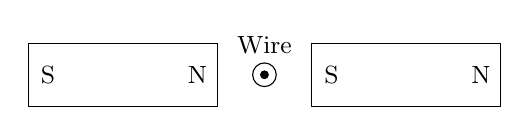
\begin{tikzpicture}
    \draw (0,0) rectangle (2.4,0.8); \node[font=\small] at (0.25,0.4) {S}; \node[font=\small] at (2.15,0.4) {N};
    \draw (3.6,0) rectangle (6.0,0.8); \node[font=\small] at (3.85,0.4) {S}; \node[font=\small] at (5.75,0.4) {N};
    \draw (3.0,0.4) circle (0.15); \fill (3.0,0.4) circle (1.6pt);
    \node[above=4pt, font=\small] at (3.0,0.4) {Wire};
  \end{tikzpicture}
\end{center}
What is the direction of the force on the wire?
\opts{Left}{Right}{Up the page}{Down the page}
\end{quizq}

% ---- Q20 (square loop in a field: axis and direction of rotation)
\Needspace{36\baselineskip}
\begin{quizq}{}
A square loop of wire lies in the plane of the page, in a uniform magnetic field directed to the right.
A current flows clockwise around the loop, as shown. $WX$ and $YZ$ are axes through the centre of the
loop.
\begin{center}
  \begin{tikzpicture}
    \foreach \y in {-1.5,-0.9,...,1.6} \draw[->, line width=0.4pt, black!60] (-2.4,\y) -- (2.4,\y);
    \node[right, font=\small] at (2.4,1.5) {$B$};
    \draw[line width=1.3pt] (-1.1,-1.1) rectangle (1.1,1.1);
    \draw[->, line width=0.8pt] (-1.1,-0.2) -- (-1.1,0.3); \draw[->, line width=0.8pt] (1.1,0.2) -- (1.1,-0.3);
    \draw[->, line width=0.8pt] (-0.2,1.1) -- (0.3,1.1); \draw[->, line width=0.8pt] (0.2,-1.1) -- (-0.3,-1.1);
    \draw[guide] (0,-2.0) -- (0,2.0); \node[above, font=\small] at (0,2.0) {$W$}; \node[below, font=\small] at (0,-2.0) {$X$};
    \draw[guide] (-2.7,0) -- (2.7,0); \node[left, font=\small] at (-2.7,0) {$Y$}; \node[right, font=\small] at (2.7,0) {$Z$};
    \node[left, font=\small] at (-1.1,0.7) {left side}; \node[right, font=\small] at (1.1,-0.7) {right side};
  \end{tikzpicture}
\end{center}
How does the loop start to move?
\begin{center}
  \renewcommand\arraystretch{1.7}
  \begin{tabular}{@{}p{10mm}|>{\centering\arraybackslash}p{38mm}|>{\centering\arraybackslash}p{56mm}|}
    \cline{2-3}
    & \textit{Axis of rotation} & \textit{Direction of movement}\\ \cline{2-3}
    A. & $YZ$ & Left side moves into the page\\ \cline{2-3}
    B. & $YZ$ & Left side moves out of the page\\ \cline{2-3}
    C. & $WX$ & Left side moves into the page\\ \cline{2-3}
    D. & $WX$ & Left side moves out of the page\\ \cline{2-3}
  \end{tabular}
\end{center}
\end{quizq}

% ---- Q21 (force per metre between parallel wires)
\Needspace{12\baselineskip}
\begin{quizq}{}
Two long parallel wires are \qty{0.50}{m} apart. One carries a current of \qty{2.0}{A} and the other
carries \qty{3.0}{A}. What is the size of the force per metre between the wires?
\opts{\qty{6.0e-7}{N.m^{-1}}}{\qty{2.4e-6}{N.m^{-1}}}{\qty{4.8e-6}{N.m^{-1}}}{\qty{1.5e-5}{N.m^{-1}}}
\end{quizq}

% ---- Q22 (expression for the separation)
\Needspace{14\baselineskip}
\begin{quizq}{}
Two parallel wires, each of length $l$, carry currents $I_1$ and $I_2$. The force between them is $F$.
Which expression gives the distance $r$ between the wires?
\opts{$\dfrac{\mu_0 I_1 I_2 l}{2\pi F}$}{$\dfrac{2\pi F}{\mu_0 I_1 I_2 l}$}{$\dfrac{\mu_0 I_1 I_2}{2\pi F l}$}
  {$\sqrt{\dfrac{\mu_0 I_1 I_2 l}{2\pi F}}$}
\end{quizq}

% ---- Q23 (force on a conductor at an angle to B)
\Needspace{26\baselineskip}
\begin{quizq}{}
A conductor of length \qty{0.080}{m} carries a current of \qty{3.0}{A}. It lies at \ang{40} to a
uniform magnetic field of \qty{0.50}{T}, as shown.
\begin{center}
  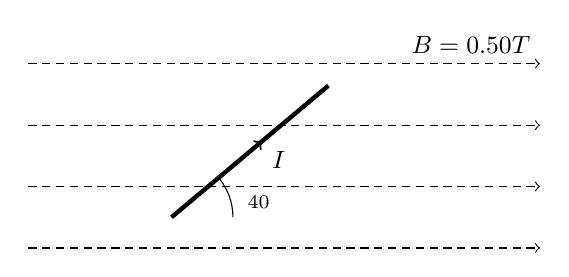
\begin{tikzpicture}[scale=1.3]
    \foreach \y in {0,0.6,...,1.9} \draw[->, line width=0.4pt, dash pattern=on 3pt off 2pt] (0,\y) -- (5,\y);
    \node[above left, font=\small] at (5,1.8) {$B = \qty{0.50}{T}$};
    \draw[line width=1.6pt] (1.4,0.3) -- ++(40:2.0);
    \draw[->, line width=0.7pt] (1.9,0.72) -- ++(40:0.5) node[below right, font=\small] {$I$};
    \draw (2.0,0.3) arc (0:40:0.6); \node[font=\scriptsize] at (2.25,0.45) {\ang{40}};
  \end{tikzpicture}
\end{center}
What is the magnitude of the force on the conductor?
\opts{\qty{0}{N}}{\qty{0.077}{N}}{\qty{0.092}{N}}{\qty{0.12}{N}}
\end{quizq}

% ---- Q24 (two wires and an electronic balance)
\Needspace{24\baselineskip}
\begin{quizq}{}
Wire $X$ is fixed in place. Wire $Y$ rests on an electronic balance directly below $X$. The two wires
carry currents in opposite directions, as shown.
\begin{center}
  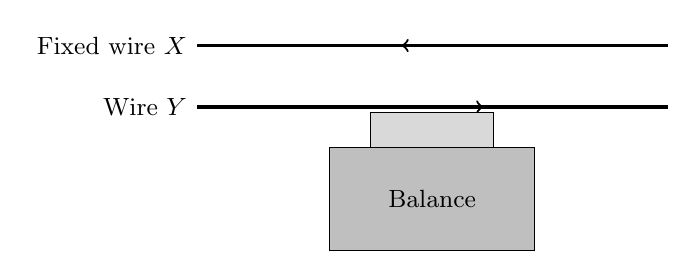
\begin{tikzpicture}[scale=1.3]
    \draw[line width=1.4pt] (0,1.6) -- (4.6,1.6); \draw[->, line width=0.8pt] (2.8,1.6) -- (2.0,1.6);
    \node[left, font=\small] at (0,1.6) {Fixed wire $X$};
    \draw[line width=1.4pt] (0,1.0) -- (4.6,1.0); \draw[->, line width=0.8pt] (2.0,1.0) -- (2.8,1.0);
    \node[left, font=\small] at (0,1.0) {Wire $Y$};
    \draw[fill=black!15] (1.7,0.95) rectangle (2.9,0.6); \draw[fill=black!25] (1.3,0.6) rectangle (3.3,-0.4);
    \node[font=\small] at (2.3,0.1) {Balance};
  \end{tikzpicture}
\end{center}
Which statement is correct?
\opts{If the current in $Y$ is reversed, the balance reading increases.}
  {The balance reading equals the mass of $Y$, because the magnetic forces cancel.}
  {If both currents are reversed, the balance reading decreases.}
  {If the current in $X$ is increased, the balance reading increases.}
\end{quizq}

% ---- Q25 (angle that halves the force)
\Needspace{13\baselineskip}
\begin{quizq}{}
A straight rod carrying a current is at right angles to a uniform magnetic field. The rod is rotated in
the plane that contains the field, so that the force on it halves. Through what angle was the rod
rotated?
\opts{\ang{30}}{\ang{45}}{\ang{60}}{\ang{90}}
\end{quizq}

% ---- Q26 (force direction with compass directions)
\Needspace{13\baselineskip}
\begin{quizq}{}
A horizontal wire runs east--west just above a magnet. At the wire, the magnet's field points
vertically upwards. A current flows in the wire from west to east. In which direction is the force on
the wire?
\opts{South}{North}{Vertically upwards}{Vertically downwards}
\end{quizq}

% ---- Q27 (net force on one of three wires)
\Needspace{28\baselineskip}
\begin{quizq}{}
$P$, $Q$ and $R$ are long straight conductors carrying currents of the same size $I$, in the directions
shown. $P$ and $Q$ are fixed. The magnitude of the force between $Q$ and $R$ alone is $F$.
\begin{center}
  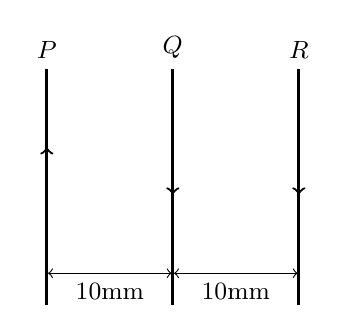
\begin{tikzpicture}
    \foreach \x/\l in {0/P, 1.6/Q, 3.2/R} {\draw[line width=1.1pt] (\x,0) -- (\x,3); \node[above, font=\small] at (\x,3) {$\l$};}
    \draw[->, line width=0.8pt] (0,1.4) -- (0,2.0); \draw[->, line width=0.8pt] (1.6,2.0) -- (1.6,1.4); \draw[->, line width=0.8pt] (3.2,2.0) -- (3.2,1.4);
    \draw[|<->|, line width=0.4pt] (0,0.4) -- (1.6,0.4) node[midway, below, font=\small] {\qty{10}{mm}};
    \draw[|<->|, line width=0.4pt] (1.6,0.4) -- (3.2,0.4) node[midway, below, font=\small] {\qty{10}{mm}};
  \end{tikzpicture}
\end{center}
What is the net force on $R$?
\opts{$\dfrac{F}{2}$ to the left}{$\dfrac{F}{2}$ to the right}{$\dfrac{3F}{2}$ to the left}{$\dfrac{3F}{2}$ to the right}
\end{quizq}

% ---- Q28 (scaling: separation and currents tripled)
\Needspace{12\baselineskip}
\begin{quizq}{}
Two parallel wires a distance $d$ apart carry equal currents. The distance is increased to $3d$, and the
current in each wire is tripled. What happens to the magnetic force between the wires?
\opts{It does not change.}{It increases by a factor of 3.}{It increases by a factor of 9.}
  {It decreases by a factor of 3.}
\end{quizq}

% ---- Q29 (current from force, with an angle)
\Needspace{12\baselineskip}
\begin{quizq}{}
A \qty{0.30}{m} length of wire lies at \ang{30} to a uniform magnetic field of \qty{0.040}{T}. The force
on the wire is \qty{0.024}{N}. What is the current in the wire?
\opts{\qty{1.0}{A}}{\qty{2.0}{A}}{\qty{2.3}{A}}{\qty{4.0}{A}}
\end{quizq}

% ---- Q30 (trolleys pushed apart)
\Needspace{14\baselineskip}
\begin{quizq}{}
Two parallel vertical wires, each \qty{1.50}{m} long, are mounted on two identical trolleys. They are
\qty{3.0}{mm} apart and carry currents of \qty{30}{A} and \qty{40}{A} in opposite directions. When the
currents are switched on, each trolley starts to move away from the other with an acceleration of
\qty{0.050}{m.s^{-2}}. Ignore friction. What is the mass of each trolley?
\opts{\qty{1.2}{kg}}{\qty{1.6}{kg}}{\qty{2.4}{kg}}{\qty{4.8}{kg}}
\end{quizq}

% ---- Q31 (field into the page: angle does not matter)
\Needspace{24\baselineskip}
\begin{quizq}{}
A conductor of length $l$ carrying a current of \qty{3.0}{A} lies in the plane of the page, at \ang{40}
to the horizontal. It is in a uniform magnetic field of \qty{0.25}{T} directed into the page.
\begin{center}
  \begin{tikzpicture}[scale=1.4]
    \fieldin{0}{0}{3.6}{1.8}{0.6}
    \draw[line width=1.4pt] (0.4,0.1) -- ++(40:2.1); \draw[->, line width=0.8pt] (1.0,0.6) -- ++(40:0.5) node[below right, font=\small] {$I$};
    \draw[guide] (0.4,0.1) -- (1.8,0.1); \draw (1.0,0.1) arc (0:40:0.6); \node[font=\scriptsize] at (1.25,0.28) {\ang{40}};
  \end{tikzpicture}
\end{center}
Which expression gives the magnitude of the force on the conductor?
\opts{$F = (0.25)(3.0)\,l$}{$F = (0.25)(3.0)\,l\sin 40^\circ$}{$F = (0.25)(3.0)\,l\cos 40^\circ$}
  {$F = (0.25)(3.0)\,l\sin 50^\circ$}
\end{quizq}

% ---- Q32 (rod suspended below another rod)
\Needspace{16\baselineskip}
\begin{quizq}{}
Rod $X$ is fixed to a support. An identical rod $Y$ hangs freely, directly below $X$, held up only by
the magnetic force between the rods. Both rods carry currents. The connecting wires have negligible
mass. Which statement must be correct?
\opts{The currents in $X$ and $Y$ are in opposite directions.}
  {The magnetic force on $X$ is upwards.}
  {The support must hold up a force equal to the total weight of $X$ and $Y$.}
  {The magnetic force on $Y$ is greater than the magnetic force on $X$.}
\end{quizq}

% ---- Q33 (magnet on a balance)
\Needspace{14\baselineskip}
\begin{quizq}{}
A magnet sits on an electronic balance, which reads \qty{0.300}{kg}. A fixed horizontal copper rod
passes between the poles of the magnet without touching it, at right angles to the field. When a
current $I$ flows in the rod, the magnetic force on the rod is vertically upwards. Which expression
gives the new balance reading?
\opts{$\qty{0.300}{kg} + BIl$}{$\qty{0.300}{kg} + \dfrac{BIl}{9.8}$}{$\qty{0.300}{kg} - BIl$}
  {$\qty{0.300}{kg} - \dfrac{BIl}{9.8}$}
\end{quizq}

% ---- Q34 (force between wires carrying AC in the same direction)
\Needspace{40\baselineskip}
\begin{quizq}{}
Two long parallel wires are connected so that they carry identical alternating currents, in the
\emph{same} direction at every instant. Which graph shows how the magnetic force between the wires
varies with time?
\gridopts{%
  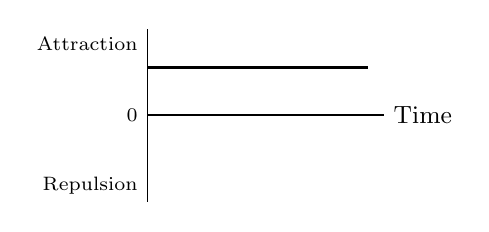
\begin{tikzpicture}
    \draw[line width=0.6pt] (0,-1.1) -- (0,1.1); \draw[line width=0.6pt] (0,0) -- (3,0) node[right, font=\small] {Time};
    \node[left, font=\scriptsize] at (0,0.9) {Attraction}; \node[left, font=\scriptsize] at (0,-0.9) {Repulsion}; \node[left, font=\scriptsize] at (0,0) {0};
    \draw[line width=1pt] (0,0.6) -- (2.8,0.6);
  \end{tikzpicture}}
  {%
  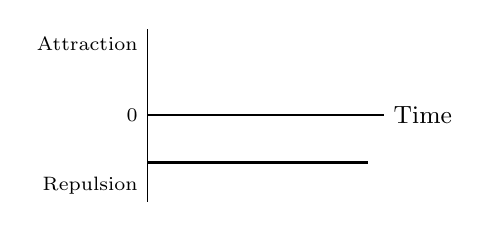
\begin{tikzpicture}
    \draw[line width=0.6pt] (0,-1.1) -- (0,1.1); \draw[line width=0.6pt] (0,0) -- (3,0) node[right, font=\small] {Time};
    \node[left, font=\scriptsize] at (0,0.9) {Attraction}; \node[left, font=\scriptsize] at (0,-0.9) {Repulsion}; \node[left, font=\scriptsize] at (0,0) {0};
    \draw[line width=1pt] (0,-0.6) -- (2.8,-0.6);
  \end{tikzpicture}}
  {%
  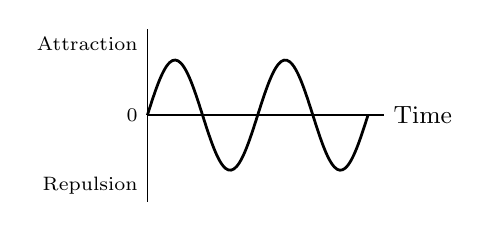
\begin{tikzpicture}
    \draw[line width=0.6pt] (0,-1.1) -- (0,1.1); \draw[line width=0.6pt] (0,0) -- (3,0) node[right, font=\small] {Time};
    \node[left, font=\scriptsize] at (0,0.9) {Attraction}; \node[left, font=\scriptsize] at (0,-0.9) {Repulsion}; \node[left, font=\scriptsize] at (0,0) {0};
    \draw[line width=1pt, domain=0:2.8, samples=80, smooth] plot (\x, {0.7*sin(257*\x)});
  \end{tikzpicture}}
  {%
  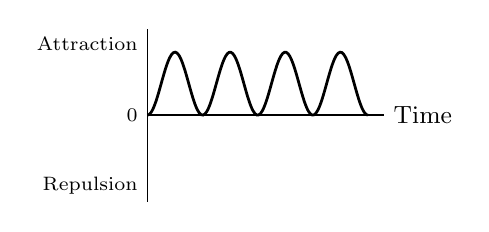
\begin{tikzpicture}
    \draw[line width=0.6pt] (0,-1.1) -- (0,1.1); \draw[line width=0.6pt] (0,0) -- (3,0) node[right, font=\small] {Time};
    \node[left, font=\scriptsize] at (0,0.9) {Attraction}; \node[left, font=\scriptsize] at (0,-0.9) {Repulsion}; \node[left, font=\scriptsize] at (0,0) {0};
    \draw[line width=1pt, domain=0:2.8, samples=120, smooth] plot (\x, {0.8*(sin(257*\x))^2});
  \end{tikzpicture}}
\end{quizq}

% ---- Q35 (Newton's third law for wires with different currents)
\Needspace{14\baselineskip}
\begin{quizq}{}
Two long parallel wires carry currents $I$ and $3I$. Which statement about the magnetic forces between
them is correct?
\opts{The forces on the two wires are equal in size and opposite in direction.}
  {The force on the wire carrying $3I$ is three times the force on the other wire.}
  {The force on the wire carrying $I$ is three times the force on the other wire.}
  {The forces on the two wires act in the same direction.}
\end{quizq}

% ---- Q36 (force on the other wire after one current is tripled)
\Needspace{30\baselineskip}
\begin{quizq}{}
Two parallel wires, $X$ and $Y$, carry currents in opposite directions. The force on wire $Y$ is
represented by the vector $F$.
\begin{center}
  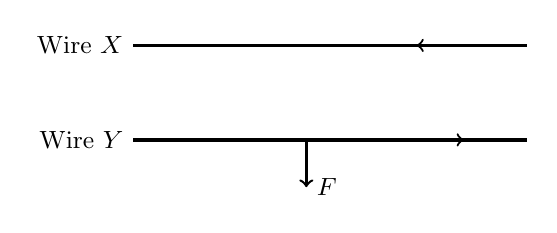
\begin{tikzpicture}
    \draw[line width=1.2pt] (0,1.2) -- (5,1.2); \draw[->, line width=0.8pt] (4.2,1.2) -- (3.6,1.2); \node[left, font=\small] at (0,1.2) {Wire $X$};
    \draw[line width=1.2pt] (0,0) -- (5,0); \draw[->, line width=0.8pt] (3.6,0) -- (4.2,0); \node[left, font=\small] at (0,0) {Wire $Y$};
    \draw[->, line width=0.9pt] (2.2,0) -- (2.2,-0.6) node[right, font=\small] {$F$};
  \end{tikzpicture}
\end{center}
The current in wire $X$ is then tripled. Its direction does not change. Which vector represents the
force on wire $X$ now? (The arrows are drawn to the same scale as $F$.)
\gridopts{\tikz{\draw[->, line width=0.9pt] (0,0.6) -- (0,0);}}
  {\tikz{\draw[->, line width=0.9pt] (0,0) -- (0,0.6);}}
  {\tikz{\draw[->, line width=0.9pt] (0,1.8) -- (0,0);}}
  {\tikz{\draw[->, line width=0.9pt] (0,0) -- (0,1.8);}}
\end{quizq}
